\documentclass[UTF8,openany]{ctexbook}

% 论文版面要求:
% 统一按 word 格式A4纸(页面设置按word默认值)编排、打印、制作。
% 正文内容字体为宋体;字号为小4号;字符间距为标准;行距为25磅(约0.88175cm)。

%%%%% ===== 页面设置
\usepackage[a4paper,top=2.54cm,bottom=2.54cm,left=3.17cm,right=3.17cm,%
            ]{geometry}
\usepackage{tcolorbox}
\usepackage{colortbl}
\usepackage{dirtree}
\usepackage{longtable}
\usepackage{booktabs}
\usepackage{subfigure}
\usepackage{multirow}
            
\setlength{\parindent}{2em}
%默认的弹性间距会导致文中某些排版flush的时候,出现大量空白。
\setlength{\parskip}{0.5em} %指定固定段后间距,默认为弹性间距。
\setlength{\intextsep}{10pt} %固定浮浮动体前后间距。
\usepackage{enumitem}
\usepackage{ulem}

%%%%% =====章节 标题 设置
\ctexset{%
  contentsname={\vspace{-3.5em}\centerline{\zihao{-3}\heiti 目\quad 录}\vspace{-0.7em}},
  listfigurename={\vspace{-3.5em}\centerline{\zihao{-3}\heiti 插\ 图\ 目\ 录}\vspace{-0.5em}},
  listtablename={\vspace{-3.5em}\centerline{\zihao{-3}\heiti 表\ 格\ 目\ 录}\vspace{-0.5em}},
  bibname={\vspace{-3em}\centerline{\zihao{-3}\heiti 参\ 考\ 文\ 献}\vspace{3em}},
  chapter={name={,},
  number=\arabic{chapter}, %指定章序号为一二三。。。。
  nameformat={\zihao{-2}\bfseries},
  titleformat={\zihao{-2}\bfseries},
  format=\raggedright,
  beforeskip={10pt},
  afterskip={10pt},
  pagestyle={fancy}
  },
section={format=\raggedright,
  nameformat={\zihao{3}\bfseries},
  titleformat={\zihao{3}\bfseries},
%           afterskip={1ex plus 0.2ex}
  beforeskip={1ex},% 固定段前段后间距,
  afterskip={1ex}
  },
subsection={format=\raggedright,
  nameformat={\zihao{-3}\bfseries},
  titleformat={\zihao{-3}\bfseries},
%           afterskip={0.5ex plus 0.1ex}
  beforeskip={0.5ex},
  afterskip={0.5ex}
  }
}
\AddToHook{package/xeCJK/after}{\defaultCJKfontfeatures{}} % 重置字体设置
%%%%% ===== 中英文字体
%\setsansfont{Myriad Pro} % 无衬线字体 sans serif \sffamily
%\setmonofont{Consolas}   % 等宽字体 typewriter \ttfamily
%\newcommand{\Times}{\fontspec{Times New Roman}}
%% 中文字体
%\setCJKmainfont[BoldFont={Microsoft YaHei},ItalicFont={KaiTi}]{NSimSun}
%\setCJKsansfont{Microsoft YaHei}
%\setCJKmonofont{KaiTi}
% \setCJKfamilyfont{STSong}{方正小标宋_GBK}\newcommand{\STSong}{\CJKfamily{STSong}}
\setCJKfamilyfont{songti}{STZhongsong}\newcommand{\STSong}{\CJKfamily{STSong}}

%%%%% ===== 常用宏包
\usepackage{amsmath,amssymb,amsfonts,bm}
\usepackage[amsmath,thref,thmmarks,hyperref]{ntheorem}
\usepackage{graphicx,xcolor,float}
\usepackage{fancyhdr}

\graphicspath{{img/}}


\usepackage{booktabs} % toprule, midrule, bottomrule
\usepackage{varwidth} % 可变宽度的 parbox

%%%%% ===== 参考文献与链接
\usepackage[numbers,sort&compress,sectionbib,super, square]{natbib} %引用上标,禁用连续缩写。
\newcommand{\upcite}[1]{\textsuperscript{\cite{#1}}}


\usepackage[xetex,pagebackref]{hyperref}
\hypersetup{CJKbookmarks=true,colorlinks=true,citecolor=blue,%
            linkcolor=blue,urlcolor=blue,bookmarksnumbered=true,%
	        bookmarksopen=true,breaklinks=true}
	        
	        
	        
\iffalse   % 调试时,可去掉,以用于显示引用位置。
\renewcommand*{\backrefalt}[4]{%
\ifcase #1 No citations.%
\or Cited on page #2.%
\else Cited on pages #2.%
%\else #1 Cited on pages #2.%
\fi
}

\else
\renewcommand*{\backrefalt}[4]{}
\fi

%%%%% ===== 浮动图表的标题
\usepackage[margin=2em,labelsep=space,skip=0.5em,font=normalfont]{caption}
\DeclareCaptionFormat{mycaption}{{\heiti\color{blue} #1}#2{\kaishu #3}}
\captionsetup{format=mycaption,tablewithin=chapter,figurewithin=chapter}%,belowskip=-10pt
%\setlength{\belowcaptionskip}{-10pt}

%%%%%% ===== 浮动图表的比例默认50%以下,否则无法浮动。
\renewcommand\floatpagefraction{.9} %当浮动体小于页面90%时进行直接放置。
\renewcommand\topfraction{.9}  
\renewcommand\bottomfraction{.9}  
\renewcommand\textfraction{.1}



%%%%% ===== 算法
\usepackage{algorithm,algpseudocode}

%%%%% ===== 其他
\usepackage{ulem}
\def\ULthickness{1pt}




%%%%%===== Code Style代码
\usepackage{listings}
\usepackage{color}

\definecolor{dkgreen}{rgb}{0,0.6,0}
\definecolor{gray}{rgb}{0.5,0.5,0.5}
\definecolor{mauve}{rgb}{0.58,0,0.82}

\usepackage{accsupp}



\newcommand\emptyaccsupp[1]{\BeginAccSupp{ActualText={}}#1\EndAccSupp{}}

\lstset{
    % language = C,
    showstringspaces=false,
    xleftmargin = 3em,xrightmargin = 3em, aboveskip = 1em,
	backgroundcolor = \color{white}, % 背景色
	basicstyle = \small\ttfamily, % 基本样式 + 小号字体
	rulesepcolor= \color{gray}, % 代码块边框颜色
	breaklines = true, % 代码过长则换行
	numbers = left, % 行号在左侧显示
	numberstyle=\emptyaccsupp,
    numbersep = 14pt, 
    keywordstyle=\color{purple}\bfseries, % 关键字颜色
    commentstyle =\color{red!50!green!50!blue!60}, % 注释颜色
    stringstyle = \color{red}, % 字符串颜色
    morekeywords={ASSERT, int64_t, uint32_t},
	% frame = shadowbox, % 用(带影子效果)方框框住代码块
	frame = single, % 用(带影子效果)方框框住代码块
	showspaces = false, % 不显示空格
	columns = fixed, % 字间距固定
  framesep=1em
} 
\lstset{
    sensitive=true,
    moreemph={ASSERT, NULL}, emphstyle=\color{red}\bfseries,
    moreemph=[2]{int64_t, uint32_t, tid_t, uint8_t, int16_t, uint16_t, int32_t, size_t}, emphstyle=[2]\color{purple}\bfseries,
    showspaces = false, % 不显示空格
    }



\newcommand{\mcc}[1]{\multicolumn{1}{c}{\underline{\makebox[10em][c]{#1}}}}
\newcommand{\mce}[1]{\multicolumn{1}{c}{\underline{\makebox[15em][l]{#1}}}}


\pagestyle{fancy}
\fancyhf{}  % 清除以前对页眉页脚的设置

\newcommand{\makeheadrule}{%% 定义页眉与正文间双隔线
    \makebox[0pt][l]{\rule[.7\baselineskip]{\headwidth}{0.3pt}}%0.4
    \rule[0.85\baselineskip]{\headwidth}{1.0pt}\vskip-.8\baselineskip}
\makeatletter
\renewcommand{\headrule}{%
    % {\if@fancyplain\let\headrulewidth\plainheadrulewidth\fi\makeheadrule}}
    {\makeheadrule}}
\makeatother
\renewcommand{\chaptermark}[1]{\markboth{\CTEXthechapter \ #1}{}}
\renewcommand{\sectionmark}[1]{\markright{\thesection \ #1}{}}
%\fancyhead[RO,LE]{{\small\songti\rightmark}}     % 节标题
%\fancyhead[RE]{{\small\songti\leftmark}}      % 章标题
\fancyhead[C]{\zihao{-4}《编译原理与技术实践》课程项目报告}
% \fancyhead[RO,LE]{$\cdot$ {\small\thepage} $\cdot$}
\fancyfoot[C]{{-\thepage-}}
%\fancyfoot[CO,CE]{{\thepage}}

\ctexset{chapter/break={}}

\begin{document}

\begin{titlepage}
    \begin{center}

        {
            \begin{figure}[H]
                \vspace{5cm}
                
\includegraphics[width=14cm]{0.png}
            \end{figure}
            \heiti\zihao{2}《编译原理与技术实践》课程项目报告\\
            \vspace{1.8em}
            
        }
        
        \zihao{3}
        \begin{tabular}{@{}l@{}}
        姓名:\underline{\makebox[5cm][c]{武泽恺}} \\[1.5ex]
        学号:\underline{\makebox[5cm][c]{10225101429}}
        \end{tabular}
        \\[8em]
        \zihao{-2}2025年6月21日
    \end{center}
    \thispagestyle{fancy}
    \fancyfoot[C]{}
\end{titlepage}
\fancyfoot[C]{-\thepage-}

\setcounter{page}{1}
\pagenumbering{roman}

\thispagestyle{fancy}
\newpage

\setcounter{page}{1}
\pagenumbering{arabic}

\zihao{4}

\chapter{项目概述}

本项目是《编译原理与技术实践》课程的核心实践任务。通过独立实现编译器的多个阶段,深入理解编译原理的核心概念和算法。

我们在章节~\ref{sec:content} 中详细介绍了项目的实现内容;在章节~\ref{sec:highlights} 总结了项目的亮点和特色;在章节~\ref{sec:test} 介绍了测试用例;最后,在章节~\ref{sec:conclusion} 中总结了本次实践项目的收获。

\chapter{实现内容}
\label{sec:content}

\section{概览}

本项目中,我们分别实现了以下编译器组件:

\begin{enumerate}[noitemsep,topsep=0pt,partopsep=0pt]
    \item \textbf{词法分析器:} \texttt{lexical-analysis/main.cpp},负责将源代码转换为记号流。
    \item \textbf{LL(1)分析器:} \texttt{LL-parser/LL1.cpp},实现了LL(1)语法分析,处理简单的文法。
    \item \textbf{SLR(1) \& LR(1)分析器:} \texttt{LR-parser/SLR.cpp},实现了SLR(1)语法分析;\texttt{LR-parser/LR1.cpp},实现了LR(1)语法分析。
    \item \textbf{语义分析器:} \texttt{semantic-analysis.cpp},负责类型检查和符号表管理。
\end{enumerate}

\section{环境配置}

表~\ref{tab:config} 列出了本项目的环境配置细节。

\begin{table}[H]
    \centering
    \caption{项目环境配置}
    \label{tab:config}
    \begin{tabular}{ll}
    \toprule
    \textbf{类别} & \textbf{配置详情} \\
    \midrule
    编程语言 & C++ \\
    编译器 & g++ 11.4.0 \\
    IDE & Visual Studio Code, CLion \\
    操作系统 & WSL2 with Ubuntu 22.04 \\
    依赖库 & \texttt{libstdc++}, C++ 标准库头文件:\\
           & \texttt{<algorithm>, <cctype>, <cstdio>, <fstream>, <unordered\_set>} \\
           & \texttt{<ios>, <iostream>, <map>, <memory>, <sstream>, <vector>} \\
           & \texttt{<stack>, <stdexcept>, <string>, <unordered\_map>} \\
    \bottomrule
    \end{tabular}
\end{table}

\section{实现细节}

\subsection{词法分析器}

这一部分中,我们需要用 C/C++ 编写一个 C 语言的语法分析器程序。代码实现位于 \texttt{lexical-analysis/main.cpp}。

\begin{enumerate}[noitemsep,topsep=0pt,partopsep=0pt]
    \item 题目中给出了C语言的语言元素集合\texttt{c\_keys.txt},我们预先加载这一文件导入到程序中的\texttt{element\_table}中(23行)。
    \item 我们使用枚举类\textbf{定义了}\texttt{TokenType}(43行),表示不同的类型;定义了\texttt{Token}类(73行),包含类型、值和映射信息。对于\texttt{Token},我们可以通过\texttt{get\_token\_type()}(56行)来查表获取其类型。
    \item 词法分析器的核心是一个自动机,\textbf{它根据当前字符和状态来决定下一个状态,并生成相应的记号}。\texttt{tokenize()}(83行)实现了具体的逻辑,能够处理标识符、常量、保留字、界符、运算符以及注释。该函数读取C代码字符流,逐个字符进行状态转换,直到识别出完整的记号,随后加入到结果列表中。最终,函数返回一个\texttt{vector<Token>},包含所有识别出的记号。
\end{enumerate}

\subsection{LL分析器(LL(1))}

这一部分中,我们需要用C/C++编写一个LL(1)解析器程序。代码实现位于 \texttt{LL-parser/LL1.cpp}。

\begin{enumerate}[noitemsep,topsep=0pt,partopsep=0pt]
    \item 首先,我们\textbf{定义了}\texttt{SymbolType}枚举类(26行),表示文法符号的类型(终结符、非终结符、$\epsilon$和\$);\texttt{Symbol}类(34行)表示文法符号;\texttt{Production}类(117行)表示文法的产生式,包括左部非终结符(\texttt{Symbol})和右部符号序列\texttt{vector<Symbol>};\texttt{Grammar}类(252行)则表示文法,包含产生式列表、文法符号集合、开始符号、First集和Follow集。\texttt{parseProductions()}函数(165行)用于从输入的文法中解析产生式,\texttt{tokenize()}函数(204行)用于将输入的代码转换为\texttt{Symbol}列表。
    \item 由于LL分析器和LR分析器都会利用到\textbf{First集}和\textbf{Follow集},因此在\texttt{Grammar}类中实现了计算First集和Follow集的函数。First集和Follow集的计算可以通过递归实现,我们编写了\texttt{computeFirst()}(296行)和\texttt{computeFollow()}函数(396行),\texttt{computeFirstSets()}(389行)和\texttt{computeFollowSets()}(452行)对每一个文法符号进行计算。\texttt{computeFirstSetForSequence()}函数(350行)则用于计算给定一串符号序列的First集。
    \item 我们定义了\texttt{LL1Grammar}类继承自\texttt{Grammar},\textbf{实现了LL(1)分析表的构建和分析逻辑}。其中,\texttt{computeParseTable()} 函数(503行)来构建分析表。\texttt{parse()} 函数(528行)来执行分析逻辑,包括栈操作、语法树(\texttt{ParseTreeNode}(229行))构建和错误处理。%TODO
\end{enumerate}

\subsection{LR分析器(SLR(1) \& LR(1))}

这一部分中,我们需要用C/C++语言编写SLR(1)或LR(1)语法分析器。代码实现位于 \texttt{LR-parser/SLR.cpp} 和 \texttt{LR-parser/LR1.cpp}。

\begin{enumerate}[noitemsep,topsep=0pt,partopsep=0pt]
    \item 首先,我们\textbf{定义了}\texttt{ActionType}枚举类(515行,\texttt{SLR.cpp}),表示LR分析表中的动作类型(移进、归约、接受和错误);\texttt{Action}类(517行)表示LR分析表中的动作,包括动作类型和编号(目标状态、产生式编号或错误编号);\texttt{Item}类(567行)表示LR项目,包括产生式和点的位置;\texttt{ItemSet}类(621行)表示LR项目集,包含项目列表和状态编号。
    \item 我们定义了\texttt{SLRGrammar}类继承自\texttt{Grammar},\textbf{实现了SLR(1)分析表的构建和分析逻辑}。其中,\texttt{closure()} 函数(650行)计算项目集的闭包,\texttt{gotoSet()} 函数(676行)计算GOTO函数,并通过\texttt{buildItemSets()}(689行)构建项目集。\texttt{computeTables()} 函数(741行)来构建\texttt{ActionTable}和\texttt{GotoTable},并通过\texttt{parse()} 函数(807行)来执行分析逻辑,进行栈操作和错误处理。%TODO
    \item \texttt{LR1Grammar}类继承自\texttt{SLRGrammar},\textbf{实现了LR(1)分析表的构建和分析逻辑}。LR(1)分析器在SLR(1)的基础上增加了对$lookahead$符号的处理,覆写\texttt{closure()} 函数(1015行,\texttt{LR1.cpp})和\texttt{computeTables()} 函数(1054行)来构建LR(1)分析表。
\end{enumerate}

\subsection{语义分析器}

这一部分中,我们需要用C/C++语言编写Translation Schema。代码实现位于 \texttt{semantic-analysis/main.cpp}。

\begin{enumerate}[noitemsep,topsep=0pt,partopsep=0pt]
    \item 首先,我们\textbf{定义了}\texttt{ValueType}枚举类(32行),表示值的类型(INT、REAL);\texttt{Value}类(40行)表示值,包括类型、名称和值本身;扩展了\texttt{Symbol}类(72行),增加类型为\texttt{Value}的\texttt{valueData}成员变量;\texttt{ProductionType}枚举类(170行)表示产生式类型(声明、赋值、表达式等);扩展了\texttt{Production}类(195行),用\texttt{ProductionType}类型的\texttt{semType}成员变量来表示语义类型。
    \item 我们基于LR分析器定义了\texttt{SemanticAnalyzer}类(747行),\textbf{实现了语义分析的核心逻辑}。在LR分析器每次进行归约时,都会调用\texttt{SemanticAnalyzer}的\texttt{executeSemanticAction()}函数(770行),根据当前的产生式类型执行相应的语义动作,如符号表管理、表达式求值、条件判断等。对于条件判断,我们编写了\texttt{ConditionState}(754行)来表示当前位于条件判断的哪个分支。最终,\texttt{outputResults()}函数(977行)会检查是否有错误发生,并输出相应的结果。
\end{enumerate}

\chapter{项目亮点}
\label{sec:highlights}

\section{写法规范与代码量}

项目中代码的规范性和可读性十分重要。本项目中,所有代码均采用统一的命名规范(例如,成员变量、成员函数均采用小驼峰命名法,全局变量和函数采用小写字母加下划线命名法),以确保代码逻辑清晰、易于理解和维护。同时,为了尽可能避免代码重复,我们在实现过程中通过继承的方式复用公共逻辑,减少了代码冗余。如,Grammar类的复用逻辑如图~\ref{fig:grammar_inheritance}所示。

\begin{figure}
\centering
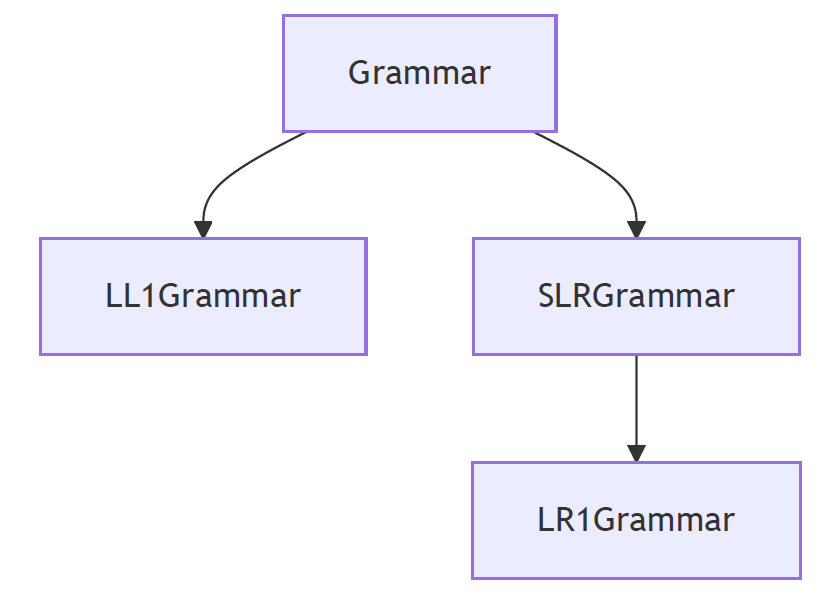
\includegraphics[width=0.5\textwidth]{extension.png}
\caption{Grammar类的继承关系}
\label{fig:grammar_inheritance}
\end{figure}

我们在实现过程中,注重代码的可读性和可维护性,确保每个模块的功能简洁、清晰且易于扩展。表~\ref{tab:code_lines} 列出了各代码文件的有效代码行数(即,不含空白行与注释行)。

\begin{table}[htbp]
\centering
\caption{各代码文件的代码行数(不含空白行)}
\label{tab:code_lines}
\begin{tabular*}{0.7\textwidth}{@{\extracolsep{\fill}}cc}
\toprule
代码文件 & 有效代码行数 \\
\midrule
词法分析 & 177 \\
LL分析器(LL(1)) & 546 \\
LR分析器(SLR(1)+LR(1)) & 993 \\
semantic-analysis.cpp & 1331 \\
\bottomrule
\end{tabular*}
\end{table}


\section{分析器实现}

在本项目中,我们遵循了编译原理课程内所学到的基本理论,完整的实现了LL分析器与LR分析器。

首先,\textbf{在 First 集与 Follow 集的计算方面},我们实现了对输入文法的自动解析机制,能够递归地计算每个非终结符的 First 集与 Follow 集。考虑到递归过程中可能出现的无限循环(特别是LR分析器没有对左递归有显式约束的情况下),我们引入了 \texttt{visited} 集合以标记已经处理过的非终结符,避免了重复计算和栈溢出。

其次,我们基于已计算的 First 集与 Follow 集,根据理论课程中的伪代码自动化构建了 LL(1) 分析表。在此基础上,LL(1) 分析器能够根据输入的终结符序列,执行语法分析过程,输出语法树以及相应的语法错误信息。

在 LR 分析器部分,\textbf{虽然课程要求我们实现SLR或LR分析器,我们考虑到于LR分析器可以在SLR分析器基础上进行增量式开发。}因此,我们按照理论课程中的伪代码实现了 SLR(1) 分析器,并进一步构建了完整的 LR(1) 分析器。这一过程中,\texttt{closure} 与 \texttt{gotoSet} 等函数均基于理论课程中的状态转移逻辑实现,完全自动化地生成 Action 表与 Goto 表。

在语义分析方面,我们基于 LR 分析器的基础,实现了符号表的管理、类型检查以及表达式求值等功能。同时,\textbf{对于SLR(1)与LR(1)分析器,我们实现了对语义分析的支持},通过在相应分析器中添加\texttt{SemanticAnalyzer}类的对象作为成员变量,便可以在每次归约时执行相应的语义动作。

因此,本项目完成了从文法描述到语法分析表构建的自动化流程,模拟了手动推导与构造的过程。

\section{信息存储结构}

表~\ref{tab:grammar_structure} 列出了各语法分析类中信息的存储结构。我们使用了 C++ 的 STL 容器(如 \texttt{unordered\_set}、\texttt{unordered\_map} 来高效地存储和管理文法符号、产生式以及分析表等信息,这些结构的底层实现基于哈希表,提供了$O(1)$的查找和插入操作。

同时,为了使用哈希表,我们为\texttt{Symbol}、\texttt{pair<int, Symbol>}、\texttt{Production}、\texttt{Item}类实现了哈希函数并重载了等于运算符,以便能够在哈希表中正确存储和比较这些对象。

\begin{table}[htbp] \small
\centering
\caption{各语法分析类中信息的存储结构}
\label{tab:grammar_structure}
\begin{tabular}{@{}ccp{5.7cm}p{3.3cm}@{}}
\toprule
\textbf{类名} & \textbf{成员变量} & \textbf{类型} & \textbf{备注} \\
\midrule

\multirow{5}{*}{\texttt{Grammar}} 
& \texttt{terminals}       & \texttt{unordered\_set<Symbol>} & 存储文法中的所有终结符符号集合 \\
& \texttt{nonTerminals}    & \texttt{unordered\_set<Symbol>} & 存储文法中的所有非终结符符号集合 \\
& \texttt{firstSets}       & \texttt{unordered\_map<Symbol, unordered\_set<Symbol>>} & 存储文法中每个符号的 First 集 \\
& \texttt{followSets}      & \texttt{unordered\_map<Symbol, unordered\_set<Symbol>>} & 存储文法中每个非终结符的 Follow 集 \\
& \texttt{productions}     & \texttt{vector<Production>} & 存储产生式 \\
\midrule

\multirow{1}{*}{\texttt{LL1Grammar}} 
& \texttt{parseTable}      & \texttt{unordered\_map<Symbol, unordered\_map<Symbol, Production>>} & 存储 LL(1) 分析表,行为非终结符,列为终结符,值为产生式 \\
\midrule

\multirow{4}{*}{\texttt{SLRGrammar}} 
& \texttt{itemSets}        & \texttt{vector<ItemSet>} & 存储 LR 项目集族 \\
& \texttt{transitions}     & \texttt{unordered\_map<int, unordered\_map<Symbol, int>>} & 状态转移表,即教科书上的\texttt{goto}函数 \\
& \texttt{actionTable}     & \texttt{unordered\_map<int, unordered\_map<Symbol, Action>>} & SLR 分析器的 ACTION 表\\
& \texttt{gotoTable}       & \texttt{unordered\_map<int, unordered\_map<Symbol, int>>} & SLR 分析器的 GOTO 表\\

\midrule

\texttt{LR1Grammar} & \multicolumn{1}{c}{/} & \multicolumn{1}{c}{/} & 完全继承自 \texttt{SLRGrammar} \\
\bottomrule
\end{tabular}
\end{table}

\section{错误处理}

本项目中,我们在LL(1)、SLR(1)/LR(1)和语义分析器支持了基本的错误处理机制。

\begin{enumerate}[noitemsep,topsep=0pt,partopsep=0pt]
    \item \textbf{LL(1)分析器:} 在\texttt{parse()}函数中,我们通过检查当前符号是否在分析表中存在来判断是否发生错误:
    \begin{itemize}[noitemsep,topsep=0pt,partopsep=0pt]
        \item 对于不匹配的终结符,直接跳过符号输出错误信息。
        \item 对于非终结符$A$,我们首先尝试采用空产生式恢复,如果该$A$的First集合包含$\epsilon$,则将当前非终结符展开为$\epsilon$,然后继续分析;否则采用Panic Mode恢复,如果当前输入也不在$A$的Follow集合中,输出错误信息并跳过当前符号;否则说明无法继续分析,输出错误信息并终止分析。
    \end{itemize}
    \item \textbf{SLR(1)/LR(1)分析器:} 根据教科书上的错误恢复方法,我们枚举错误类型来填充\texttt{ActionTable}中的错误动作。其中包括:输入符号错误地读入\texttt{\}}、\texttt{+}等表达式符号或\texttt{ID}时,将实现插入恢复(插入\texttt{;}、\texttt{ID}或\texttt{+});错误地读入\texttt{;}或右括号(\texttt{]}、\texttt{)})时,将实现删除恢复并继续分析。共\texttt{ActionTable}中填充了5种错误动作。
    \item \textbf{语义分析器:} 在语义分析过程中,我们在执行语义动作时检查是否存在类型错误、未声明的变量等问题。如果发现错误,直接输出错误信息加入到错误列表中,并在分析结束后输出所有错误信息。
    
\end{enumerate}

\chapter{测试用例}
\label{sec:test}

在这一部分中,我们介绍了在头歌测试用例的基础上,额外编写的3个测试用例,以验证其正确性。由于篇幅限制,对于每个部分,我们仅展示一个测试用例,更多的用例可以在\texttt{test}目录下找到。

\section{验证Grammar基础性功能}
\label{sec:test_grammar}

为了验证我们实现的语法分析器的基础功能,即计算First集合、Follow集合的结果是否正确,我们编写了多个测试文法来验证。

\begin{lstlisting}[caption={测试文法},label={lst:grammar_test}]
S -> A ;
A -> B A'
A' -> + B A' | E
B -> C B'
B' -> * C B' | E
C -> ( A ) | id | num
\end{lstlisting}

对于上述文法,我们通过手动计算得到结果,可以验证与我们的代码计算结果一致:

\begin{lstlisting}[caption={First集与Follow集},label={lst:first_follow}]
Symbol   First Set         Follow Set
------------------------------------------
S        ( ID NUM          $
A        ( ID NUM          ) ;
A'       + E               ) ;
B        ( ID NUM          ) ; +
B'       * E               ) ; +
C        ( ID NUM          ) ; + *
\end{lstlisting}

\section{验证LL(1)分析器}

我们仍以文法~\ref{lst:grammar_test}为例,验证LL(1)分析器的正确性。我们手动计算得到LL(1)分析表如表~\ref{tab:parse-table}所示,可以验证一致。

\begin{table}[H]
    \small
    \centering
    \caption{文法~\ref{lst:grammar_test}的LL(1)分析表}
    \label{tab:parse-table}
    \begin{tabular}{|c|c|c|c|c|c|}
        \hline
        \textbf{非终结符} & \textbf{(} & \textbf{)} & \textbf{+} & \textbf{*} & \textbf{;} \\
        \hline
        \textbf{C} & C $\to$ ( A ) & & & & \\
        \hline
        \textbf{B'} & & B' $\to$ E & B' $\to$ E & B' $\to$ * C B' & B' $\to$ E \\
        \hline
        \textbf{S} & S $\to$ A ; & & & & \\
        \hline
        \textbf{B} & B $\to$ C B' & & & & \\
        \hline
        \textbf{A'} & & A' $\to$ E & A' $\to$ + B A' & & A' $\to$ E\\
        \hline
        \textbf{A} & A $\to$ B A' & & & & \\
        \hline
    \end{tabular}
\end{table}

\section{验证LR(1)分析器}
我们也使用文法~\ref{lst:grammar_test}来验证LR(1)分析器的正确性。我们手动计算得到LR(1)分析表如表~\ref{tab:lr1-table}所示,可以验证一致。

\begin{table}[H]
\small
\centering
\caption{文法~\ref{lst:grammar_test}的LR(1)分析表}
\label{tab:lr1-table}
\begin{longtable}{|c|c|c|c|c|c|c||c|c|c|c|c|}
    \hline
    \textbf{State} & \textbf{id} & \textbf{num} & \textbf{(} & \textbf{)} & \textbf{+} & \textbf{;} & \textbf{S} & \textbf{A} & \textbf{B} & \textbf{C} & \textbf{A'} \\
    \hline
    0  & s7  & s5  & s6  &     &     &     & 2 & 1 & 3 & 4 &   \\
    1  &     &     &     &     &     & s8  &   &   &   &   &   \\
    2  &     &     &     &     &     &     &   &   &   &   &   \\
    3  &     &     &     & r4  & s9  & r4  &   &   &   &   & 10 \\
    4  &     &     &     & r7  &     & r7  &   &   &   &   &   \\
    5  &     &     &     & r10 & r10 & r10 &   &   &   &   &   \\
    6  & s7  & s5  & s6  &     &     &     &   & 13 & 3 & 4 &   \\
    7  &     &     &     & r9  & r9  & r9  &   &   &   &   &   \\
    8  &     &     &     &     &     & r1  &   &   &   &   &   \\
    9  & s7  & s5  & s6  &     &     &     &   &   & 14 & 4 &   \\
    10 &     &     &     & r2  &     & r2  &   &   &   &   &   \\
    11 &     &     &     & r5  & r5  & r5  &   &   &   &   &   \\
    12 & s7  & s5  & s6  &     &     &     &   &   &   & 15 &   \\
    13 &     &     &     & s16 &     &     &   &   &   &   &   \\
    14 &     &     &     & r4  & s9  & r4  &   &   &   &   & 17 \\
    15 &     &     &     & r7  & r7  & r7  &   &   &   &   &   \\
    16 &     &     &     & r8  & r8  & r8  &   &   &   &   &   \\
    17 &     &     &     & r3  & r3  &     &   &   &   &   &   \\
    18 &     &     &     & r6  & r6  & r6  &   &   &   &   &   \\
    \hline
\end{longtable}
\end{table}

\chapter{总结与展望}
\label{sec:conclusion}

本次编译原理实践项目让我对编译器有了更深入的理解。通过独立实现语法分析、LL(1)、SLR(1)、LR(1)和语义分析,最终成品代码数千行,不仅巩固了理论知识,也锻炼了解决复杂问题的能力。

\bibliographystyle{plain}
\bibliography{reference}

\end{document}